% -*- coding: utf-8; ispell-dictionary: "french"; -*-

%----------------------------
% Chapter 1 - Fragment Scade
%----------------------------


Scade a été développé par le laboratoire Verimag à partir des travaux sur
le langage synchrone Lustre, puis repris par la société Esterel Technologies \cite{Estech}. On retrouve
ainsi les notions de Lustre dans le langage de Scade, un programme est découpé
en noeuds dont les entrées et sorties sont des \emph{flux de données}. Ces
noeuds sont les composants que nous voulons traduire. 
Les noeuds Scade considérés dans le cadre du projet \cercles  sont
soumis à quelques restrictions. En effet, il faut limiter le langage
utilisé, car certains éléments du langage sont spécifiques aux
langages synchrones et ne sont donc pas traduisibles en B.\\

% SECTION 1 : Présentation

\section{Architecture d'un composant Scade}

\paragraph{}
Scade étant un environnement de programmation par schémas-blocs, on
développe avec des "boîtes". Par exemple, un programme d'addition sur deux flux d'entiers A
et B ayant pour sortie un flux C s'écrit:

\begin{figure}[h]
\begin{center}
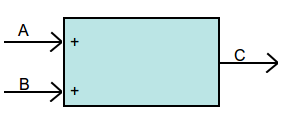
\includegraphics[scale=0.54]{1_add.png}
\end{center}
\caption{Schéma-block de l'addition}
\end{figure}

La version de ce programme correspond au noeud \texttt{add} suivant:

\begin{figure}[h]
\begin{center}
\begin{verbatim}
node add (A:int, B:int) returns (C:int);
let 
    C = A+B;
tel
\end{verbatim}
\end{center}
\caption{Version tectuelle}
\end{figure}

\paragraph{}
Au niveau des types de données utilisées, on pourra manipuler
des entiers, réels et booléens. On pourra également manipuler des
tableaux de ces types. En revanche, les types définis par
l'utilisateur tels que les types enregistrement ne seront pas gérés
par le traducteur.\\
Le comportement du noeud est ensuite défini par une liste d'équations,
dont l'ordre n'a pas d'importance. Ces équations sont de la forme:
\begin{verbatim}
left_part = expr;
\end{verbatim}
Où \texttt{left\_part} désigne une variable locale ou une sortie du composant, et expr
est une expression portant sur une ou plusieurs variables locales ou entrées.

\paragraph{}
Les expressions disponibles sont toutes les expressions arithmétiques
(\texttt{+, -, /, *, mod}), les expressions relationnelles (\texttt{<, >, <=, >=, =, <>})
et logiques (\texttt{and, or, xor, not}). Les expressions conditionelles sont également
possibles (\texttt{if .. then .. else ..}). Sont également disponibles les opérations sur les tableaux, telles que
la définition, l'index, et la concaténation.\\
Enfin, on peut évidemment faire des appels à d'autres
noeuds, pour mettre en pratique la notion de composant réutilisable. \\



% SECTION 2 : Restrictions

\section{Le temps avec Scade}

Le temps est un élément primordial dans ces systèmes dits "réactifs", où
l'on manipule des flux de données. Le temps est discrétisé en instants,
et chaque instant correspond à 1 tic de l'horloge de base. A chaque
instant i, les équations du noeud sont résolues à partir du flux reçu
en entrée à cet instant, et produit le flux de sortie correspondant au
résultat au même instant.

\paragraph{Une horloge unique}
Avec les langages synchrones, on peut
synchroniser des instructions sur des horloges différentes. On utilise des
opérateurs spécifiques au temps pour synchroniser une instruction sur une
horloge spécifique. Pour assurer la bonne définition des noeuds dont les
instructions sont calculées sur des horloges différentes, il existe

A COMPLETER AVEC ARTICLE POUZET

Cependant, dans le cadre de ce projet, nous n'utiliserons qu'une seule horloge,
celle de base. Toutes les équations sont résolues au même instant. 
Le seul opérateur temporel utilisable est l'opérateur \texttt{fby}. 

\paragraph{L'opérateur fby}

\begin{itemize}
\item pre X donne la valeur de l'expression X à l'instant précédent. A
l'instant 0 \footnote{On suppose que le premier instant est l'instant
0}, la valeur de pre X n'est pas définie. 
\item A -> B donne au premier instant la valeur de l'expression A, 
puis la valeur de l'expression B pour les instants allant de 1 à n. 
\end{itemize}

Cette construction correspond au bloc Simulink 1/Z, où A représente un
flux constant qui donnera la valeur de sortie à l'instant 0 du
bloc. Puis pour les instants 1 à n, on aura la valeur de l'expression
X à l'instant (1 à n)-1. \\
On appellera cette construction un \emph{registre}, qui est initialisé avec la
valeur A, et qui permet d'accéder à la valeur précédente de X à tout
instant. Cette construction permet de donner un \emph{état} à un composant.


\section{Contrats}

\paragraph{Assertions}
On peut définir des assertions dans un noeud afin de poser des
restrictions sur les valeurs d'entrée ou de sortie du composant. Avec
Scade, ces assertions sont possibles avec :
\begin{itemize}
\item \texttt{assume A: expr}, où \texttt{A} correspond à l'identifiant de la condition, et
\texttt{expr} un prédicat portant sur une entrée du noeud.
\item \texttt{guarrantee G: expr}, où \texttt{G} est l'identifiant de la condition, et
\texttt{expr} un prédicat portant sur une sortie du noeud.
\end{itemize}
Ces assertions forment le contrat du composant, et seront
obligatoires sauf pour la restriction sur les booléen qui est triviale (la
valeur sera vraie ou fausse).\\
Par exemple, en reprenant le noeud \texttt{add} précédent, on impose comme condition sur
les entrées qu'elles doivent être comprises entre 0 et 100 inclus. Si les
préconditions sont respectées, alors la sortie sera comprise entre 0 et 200 inclus:
\begin{verbatim}
node add (A:int, B:int) returns (C:int);
let 
    assume A_1 : A <= 100 & A >= 0;
    assume A_2 : B <= 100 & B >= 0;
    guarantee G_1 : C <= 200 & C >= 0;
    C = A+B;
tel
\end{verbatim}

